\chapter{Beschreibung des aktuellen Prozesses}\label{ch:prozessbeschreibung}


\section{\gls{erp}-Systeme als Datenquelle des Process Mining}\label{sec:erp-grundlagen}

Um den Untersuchungsgegenstand einzuordnen, sind einige Grundbegriffe zu klären. Ein Anwendungssystem besteht aus \gls{it}-Infrastruktur, Anwendungssoftware und Daten \parencite[Folie~16]{coletta2026_0303}. Anwendungssysteme lassen sich nach Organisationsebenen unterscheiden: Auf der operativen Ebene führen sie die täglichen Routinetransaktionen aus und zeichnen sie auf, darüber liegen Management-Informationssysteme für Standardberichte sowie Entscheidungs- und Führungsunterstützungssysteme für schwächer strukturierte Entscheidungen \parencite[Folie~33--39]{coletta2026_0303}. \gls{erp}-Systeme sind der prototypische Vertreter der operativen Ebene, und weil dort jede Transaktion protokolliert wird, entsteht dort auch das Rohmaterial für spätere Analysen.

Der Begriff \gls{erp} ist historisch gewachsen. Aus einfachen Systemen der Materialbedarfsplanung (MRP) entwickelte sich über die Zwischenstufe MRP\,II die integrierte Unternehmensplanung, die Vertrieb, Finanzwesen, Warenwirtschaft und Controlling zusammenführte \parencite[Folie~43]{coletta2026_0303}. Entscheidend für die vorliegende Arbeit ist die Integration: Betriebliche Anwendungssysteme lassen sich horizontal, entlang der Prozesskette über Funktionsbereiche hinweg, und vertikal, über die Führungsebenen, integrieren, und diese Integration setzt eine gemeinsame Datenhaltung voraus \parencites[S.~4]{gronau2014erp}[Folie~44 und 48]{coletta2026_0303}. Ein wesentlicher Nutzen von \gls{erp}-Systemen besteht denn auch darin, dass sich Informationssilos öffnen und vormals getrennte Teilprozesse miteinander verzahnt werden \parencite[Folie~74]{coletta2026_1003}.

Für Process Mining ist diese Eigenschaft fundamental. Weil ein Kundenauftrag nicht in mehreren getrennten Abteilungssystemen, sondern in einer integrierten Datenbank abgewickelt wird, hinterlässt er dort seine vollständige, lückenlose Spur, vom ersten Beleg bis zum Zahlungsausgleich. Ohne diese Integration wäre die Rekonstruktion eines durchgängigen Prozessablaufs praktisch unmöglich, mit ihr wird sie zur reinen Datenextraktionsaufgabe. Das \gls{erp}-System ist damit nicht nur das System, das den Prozess ausführt, sondern zugleich das System, das ihn dokumentiert. Ergänzend ist \gls{erp}-Software Standardsoftware mit vordefinierten, an Best Practices orientierten Geschäftsprozessen, die per Customizing an das Unternehmen angepasst werden \parencite[Folie~41]{coletta2026_0303}. Zwei Unternehmen mit derselben Software können daher völlig unterschiedliche Ist-Prozesse aufweisen, nicht weil die Software verschieden wäre, sondern weil sie unterschiedlich konfiguriert und genutzt wird. Genau diese Lücke zwischen vorgesehenem Standard und tatsächlicher Nutzung ist der Gegenstand der Fit/Gap-Analyse in Kapitel~\ref{ch:fitgap}, für die Process Mining die empirische Grundlage liefert.

Diese integrierte Datenhaltung unterscheidet operative \gls{erp}-Systeme grundlegend von analytischen Systemen wie einem Data Warehouse, das Daten für Auswertungszwecke aus den operativen Beständen extrahiert und aufbereitet. Process Mining nimmt eine Zwischenstellung ein: Es wertet operative Belegdaten aus, benötigt dafür aber, ähnlich einem Data-Warehouse-Ladeprozess, einen vorgeschalteten Extraktions- und Aufbereitungsschritt \parencite[Folie~400 f.]{coletta2026_2306}. Genau dieser Schritt, die Rekonstruktion eines Event-Logs aus den Belegtabellen, steht im Zentrum von Kapitel~\ref{sec:datenstrukturen}.


\section{Der \gls{o2c}-Prozess und seine typischen Schwachstellen}\label{sec:o2c-schwachstellen}

Der untersuchte Prozess folgt dem klassischen Ablauf der Auftragsabwicklung. Ein eingehender Kundenauftrag wird im Vertriebsinnendienst erfasst, durchläuft eine Kreditprüfung, wird zur Logistik freigegeben, dort kommissioniert und mit Warenausgang ausgeliefert, anschließend fakturiert und durch den Zahlungseingang abgeschlossen \parencite[Folie~62 f.]{coletta2026_0303}. Abbildung~\ref{fig:o2c-prozess-stoerungsmuster} zeigt den Prozess mit sechs in der betrieblichen Praxis immer wieder beobachteten Störungsmustern: nachträgliche Auftragsänderungen mit Klärungsschleifen (K1) \parencites[S.~55]{adolfsson2026o2c}[S.~109 f.]{nadukuru2024o2c}, manuelle Kreditprüfungen mit Liegezeiten (K2) \parencites[S.~63 ff.]{scheibler2021vertrieb}[S.~3 ff.]{reinkemeyer2020processmining}, Liefersperren infolge lückenhafter Kundenstammdaten (K3) \parencites[S.~55 f.]{adolfsson2026o2c}[S.~63 ff.]{scheibler2021vertrieb}, Fakturierung nur im wöchentlichen Sammellauf (K4) \parencites[S.~109 f.]{nadukuru2024o2c}[S.~3 ff.]{reinkemeyer2020processmining}, Fakturasperren durch manuell im Auftrag geänderte Preise (K5) \parencites[S.~55 f.]{adolfsson2026o2c}[S.~63 ff.]{scheibler2021vertrieb} sowie Reklamationen mit Gutschrift und Nachlieferung nach Falschlieferungen (K6) \parencites[S.~21 ff.]{peters2019processmining}[S.~109 f.]{nadukuru2024o2c}. Diese sechs Muster bilden die Grundwahrheit der Untersuchung. Sie werden kontrolliert injiziert (Kapitel~\ref{sec:datengrundlage}) und müssen in Kapitel~\ref{ch:fitgap} wiedergefunden und quantifiziert werden.

\begin{figure}[!htb]
\centering
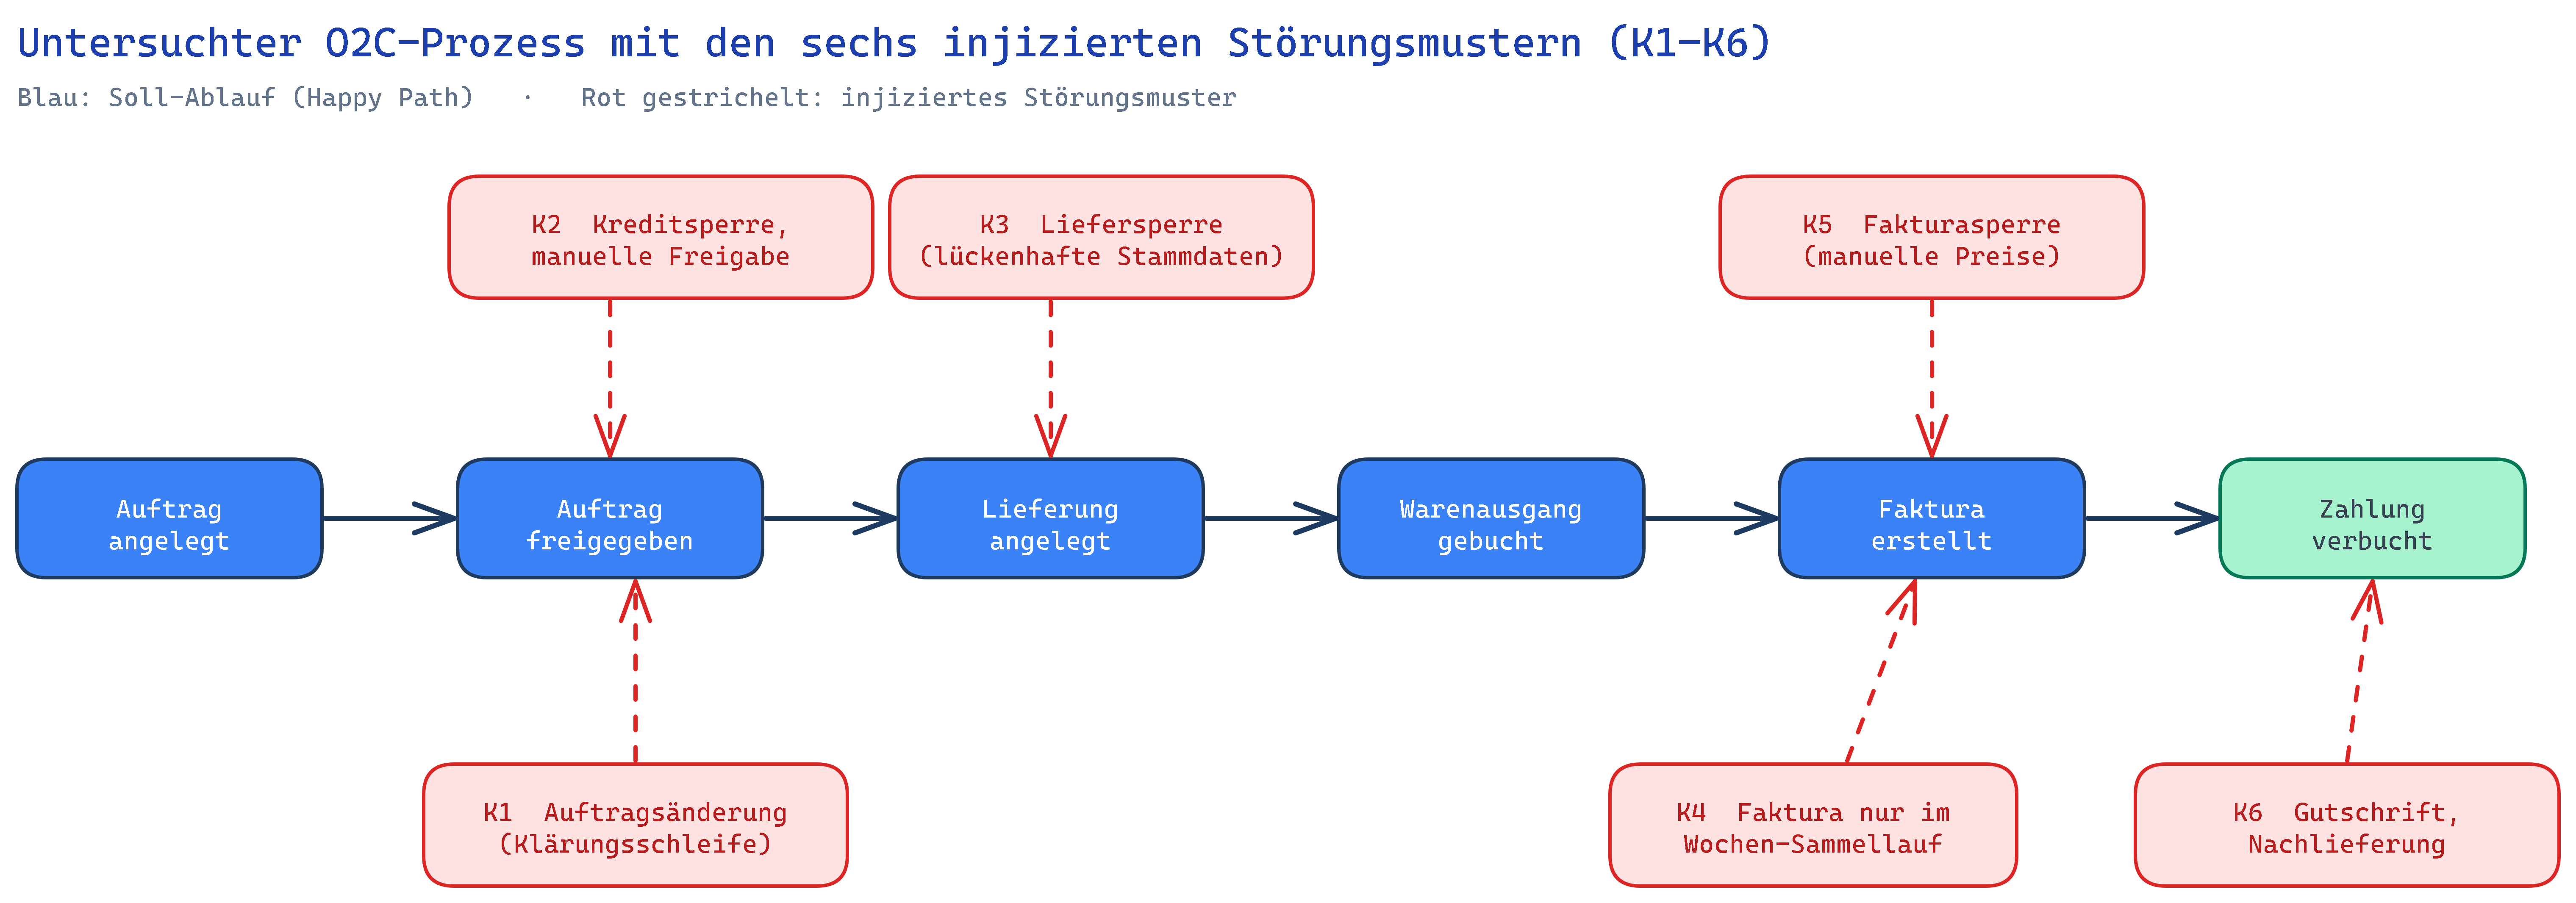
\includegraphics[width=\textwidth,height=0.36\textheight,keepaspectratio]{figures/image1.png}
\caption{Untersuchter O2C-Prozess mit den sechs injizierten Störungsmustern K1--K6 (Quelle: eigene Darstellung)}\label{fig:o2c-prozess-stoerungsmuster}
\end{figure}

Jedes dieser Muster ist für sich genommen harmlos und oft sogar gut gemeint, denn eine Kreditprüfung schützt vor Forderungsausfällen und eine Liefersperre vor Fehllieferungen. Problematisch werden sie erst durch ihre Häufigkeit und durch die Liegezeiten, die sie erzeugen. Genau diese quantitative Dimension, wie oft ein Muster auftritt, wie viel Zeit es kostet und welche Fälle betroffen sind, lässt sich in Workshops nicht zuverlässig erheben, wohl aber aus den Zeitstempeln des \gls{erp}-Systems messen. Der Beitrag des Process Mining liegt somit weniger im Entdecken der Existenz solcher Muster als in ihrer objektiven Vermessung und Priorisierung.

Ein Beispiel verdeutlicht das Zusammenspiel der Muster. Ein Bestandskunde bestellt freitags dringend benötigte Ware. Der Auftrag wird noch am selben Tag erfasst, läuft jedoch in die Kreditsperre (K2), weil ein statisches Limit rechnerisch überschritten ist. Die manuelle Freigabe erfolgt erst am Montag, die Lieferung verlässt das Werk am Mittwoch, und die Rechnung entsteht erst im Sammellauf der Folgewoche (K4). Zwischen Bestellung und Faktura vergehen so über zehn Kalendertage, ohne dass ein Beteiligter einen Fehler gemacht hätte. Die Verzögerung ist vollständig prozess- und konfigurationsbedingt und damit genau die Art von Ineffizienz, die eine datenbasierte Analyse sichtbar und messbar macht.

Kennzeichnend für den \gls{o2c}-Prozess ist zudem seine abteilungsübergreifende Natur. Der Vertrieb verantwortet Auftragserfassung und Freigabe, das Lager Kommissionierung und Warenausgang, die Finanzbuchhaltung Faktura, Zahlungseingang und Mahnwesen. Jeder Übergang zwischen diesen Bereichen ist eine potenzielle Bruchstelle, an der Wartezeiten, Rückfragen oder Medienbrüche entstehen. Gerade weil kein einzelner Bereich den Gesamtprozess überblickt, entzieht sich dessen tatsächlicher Verlauf der Wahrnehmung der Beteiligten, und gerade deshalb ist eine systemübergreifende, datenbasierte Rekonstruktion so aufschlussreich.

\section{Datengrundlage -- öffentliche und synthetische Event-Logs}\label{sec:datengrundlage}

Öffentliche Real-Logs wie der \gls{bpi}-Challenge-2019-Log erlauben Process-Mining-Untersuchungen ohne Zugriff auf vertrauliche Unternehmensdaten. Dieser dokumentiert den Bestellabwicklungsprozess (Purchase-to-Pay) eines multinationalen Konzerns mit rund 1,6 Millionen Ereignissen zu etwa 250.000 Bestellpositionen \parencite{vandongen2019bpi}. Für die vorliegende Fragestellung ist er nur eingeschränkt geeignet, weil er den Einkaufs- und nicht den Vertriebsprozess abbildet und die tatsächlichen Prozessschwächen des anonymen Konzerns unbekannt sind, eine Validierung gegen eine Grundwahrheit also unmöglich ist. Die Analyse realer Firmendaten, wie sie die \gls{o2c}-Fallstudie von Adolfsson/Saleh am Lebensmittelkonzern Paulig durchführt, erfordert wiederum genau den vertraulichen Zugang, den diese Arbeit meidet, und besitzt ebenfalls keine bekannte Grundwahrheit \parencite[S.~4 ff.\ und 28]{adolfsson2026o2c}.

Die Arbeit nutzt daher einen synthetischen \gls{sap}-\gls{o2c}-Event-Log, der mit einem Python-Simulationsskript erzeugt und mit der Open-Source-Bibliothek \gls{pm4py} verarbeitet wird \parencite{berti2019pm4py}. Simuliert werden 12.000 Kundenaufträge eines Geschäftsjahres (01.07.2025 bis 30.06.2026) entlang des \gls{sap}-Belegflusses aus Kapitel~\ref{ch:sap-prozessanalyse}, wobei die sechs Störungsmuster aus Abbildung~\ref{fig:o2c-prozess-stoerungsmuster} mit festen Wahrscheinlichkeiten und Verzögerungsverteilungen injiziert werden (Parameter in Anhang A2). Der resultierende Log umfasst 84.121 Ereignisse zu elf Aktivitätstypen und wird als \gls{csv}-Tabelle und im \gls{xes}-Format exportiert. Durch den festen Zufalls-Seed 42 ist das Vorgehen vollständig reproduzierbar, es erfordert keine Firmenfreigabe und wirft keine Datenschutzfragen auf, weil alle Benutzerkennungen synthetisch sind. An die Stelle des in der Aufgabenstellung skizzierten fiktiven Unternehmens tritt damit bewusst ein offengelegter, reproduzierbarer Datensatz, die vorgegebene Kapitelstruktur bleibt davon unberührt. Der Preis ist, dass der Log modelliertes und kein real gewachsenes Verhalten zeigt, worauf in Kapitel~\ref{ch:zusammenfassung} zurückzukommen ist.

Methodisch wird jedes Störungsmuster als bedingte Verzweigung in den Generierungsprozess eingebaut. Mit der jeweiligen Wahrscheinlichkeit aus Anhang A2 wird pro Fall entschieden, ob etwa eine Kreditsperre gesetzt wird, und die zugehörige Liegezeit wird aus einer Lognormalverteilung über Arbeitstage gezogen, sodass sich realistische, rechtsschiefe Wartezeiten mit vielen kurzen und wenigen sehr langen Verzögerungen ergeben. Weil die Wahrscheinlichkeiten und Verteilungen bekannt sind, ist die erwartete Häufigkeit jedes Musters vorab bestimmbar, und die spätere Analyse muss diese Erwartung reproduzieren, andernfalls wäre entweder die Extraktion oder der Algorithmus fehlerhaft. Der synthetische Log erfüllt damit zugleich die Rolle eines Testfalls mit bekanntem Sollergebnis.

\section{Analyse der involvierten Stammdaten und Bewegungsdaten}\label{sec:stammdaten-bewegungsdaten}

Die Daten eines Anwendungssystems lassen sich in Stammdaten, Bewegungsdaten und Organisationsdaten unterteilen \parencite[Folie~16]{coletta2026_0303}. Stammdaten sind langlebige, zustandsorientierte Daten, die über viele Geschäftsvorfälle hinweg unverändert genutzt werden, Bewegungsdaten entstehen dagegen vorgangsbezogen mit jedem einzelnen Geschäftsvorfall \parencites[Folie~322]{coletta2026_0206}[S.~165 ff.]{gronau2014erp}. Tabelle~\ref{tab:stamm-bewegungsdaten} ordnet die im \gls{o2c}-Prozess involvierten Daten dieser Klassifikation zu. Bereits diese Bestandsaufnahme zeigt, wo Prozess- und Datenqualität zusammenhängen. Dubletten im Kundenstamm, ungepflegte Versanddaten oder Sonderpreise, die statt im Konditionsstamm direkt im Auftrag gepflegt werden, erzeugen die Sperren- und Klärungsmuster K2, K3 und K5. Geringe Datenqualität schlägt zudem nach dem \gls{gigo}-Prinzip unmittelbar auf jede datengetriebene Auswertung durch \parencite[Folie~314 ff.]{coletta2026_1905}. In \gls{sap} werden Stammdaten wie der als Geschäftspartner geführte Kundenstamm oder der in funktionale Sichten gegliederte Materialstamm zentral gepflegt und von zahlreichen Belegen gemeinsam genutzt, sodass sich ein einziger unvollständiger Datensatz auf viele Vorgänge auswirkt. Stammdatenqualität ist damit doppelt relevant, als Ursache der Prozessprobleme und als Voraussetzung ihrer verlässlichen Messung.

\begin{table}[!htb]
\centering
\caption{Stamm-, Bewegungs- und Organisationsdaten im \gls{o2c}-Prozess}\label{tab:stamm-bewegungsdaten}
\small
\begin{tabularx}{\textwidth}{@{}l Y Y@{}}
\toprule
\textbf{Datenklasse} & \textbf{Beispiele im O2C-Prozess} & \textbf{Relevanz für die Prozessanalyse} \\
\midrule
Stammdaten & Kundenstamm (Adressen, Zahlungs- u. Versandbedingungen, Incoterms), Materialstamm, Preis-/\allowbreak{}Konditionsstamm, Kreditstammdaten & Fehlende oder veraltete Attribute lösen Sperren und Klärungen aus (K2, K3, K5) \\
Bewegungsdaten & Angebote, Kundenaufträge, Lieferbelege, Warenausgangsbuchungen, Fakturen, Gutschriften, Zahlungseingänge & Tragen Zeitstempel und Nutzerkennung, Rohmaterial des Event-Logs \\
Organisationsdaten & Verkaufsorganisation, Vertriebsweg, Sparte, Werk, Versandstelle, Buchungskreis & Legen Zuständigkeiten fest und ermöglichen Filterung und Vergleich von Prozessvarianten \\
\bottomrule
\end{tabularx}
\end{table}

Zusammengefasst liefert die Datenperspektive bereits einen ersten Hinweis auf die späteren Befunde: Die Bewegungsdaten machen den Prozess über ihre Zeitstempel überhaupt erst messbar, und die Stammdaten entscheiden darüber, wie störungsanfällig er verläuft. Beide Datenklassen sind damit nicht nur Gegenstand der Beschreibung, sondern die eigentlichen Stellhebel, an denen die Analyse in Kapitel~\ref{ch:fitgap} und die Maßnahmen in Kapitel~\ref{ch:anpassung} ansetzen.
